\chapter{Wstęp}
\label{cha:wstep}
Świat się zmienia. I jak jeszcze do niedawna ogólnie rozumiany postęp był postrzegany przez pryzmat nowinek technicznych ułatwiających – w mniejszym bądź większym stopniu – codzienne czynności, tak od pewnego czasu niezwykle ważną kwestią stała się ekologia. Wkrada się ona do niemal każdego aspektu naszego życia: od naklejek na sprzęcie AGD informującym o efektywności energetycznej danego urządzenia, przez powszechne i coraz bardziej rygorystyczne normy emisji silników spalinowych, po ograniczenia w spalaniu opału w prywatnych piecach. Fala „pro eko” nabiera mocy z każdym rokiem, co jest jak najbardziej zrozumiałe w kontekście zmian do jakich dochodzi na Ziemi z powodu działalności energetycznej człowieka. Jednym z ogromnej liczby postulatów ruchu proekologicznego jest ograniczenie ruchu samochodowego, zwłaszcza tego na krótki dystans. Co więc w zamian? Odpowiedź jest prosta: niemal w stu procentach ekologiczny rower. Ten wymaga jednak odpowiedniej infrastruktury oraz nieco zmiany w podejściu do kwestii transportu. \newline
Jednak trend ten jest widoczny już do dłuższego czasu: rower coraz częściej jest wybierany jako środek transportu. Co oczywiste w większości przypadków na niedługich trasach wewnątrz miejskich, jak przejazd do i z miejsca pracy lub sklepu. Wyraźnie to widać na wykresie natężenia ruchu rowerowego (Rys. 2.1.)  na jednym z głównych węzłów komunikacyjnych Krakowa (również pod względem rowerowym), czyli na Rondzie Mogilskim. Otóż wg danych Urzędu Miasta Krakowa największą liczbę rowerzystów można zaobserwować w godzinach szczytu, co jasno pokazuje, że są to w dużej mierze ludzie dojeżdżający do i z pracy.
\begin{figure}[H]
\centering
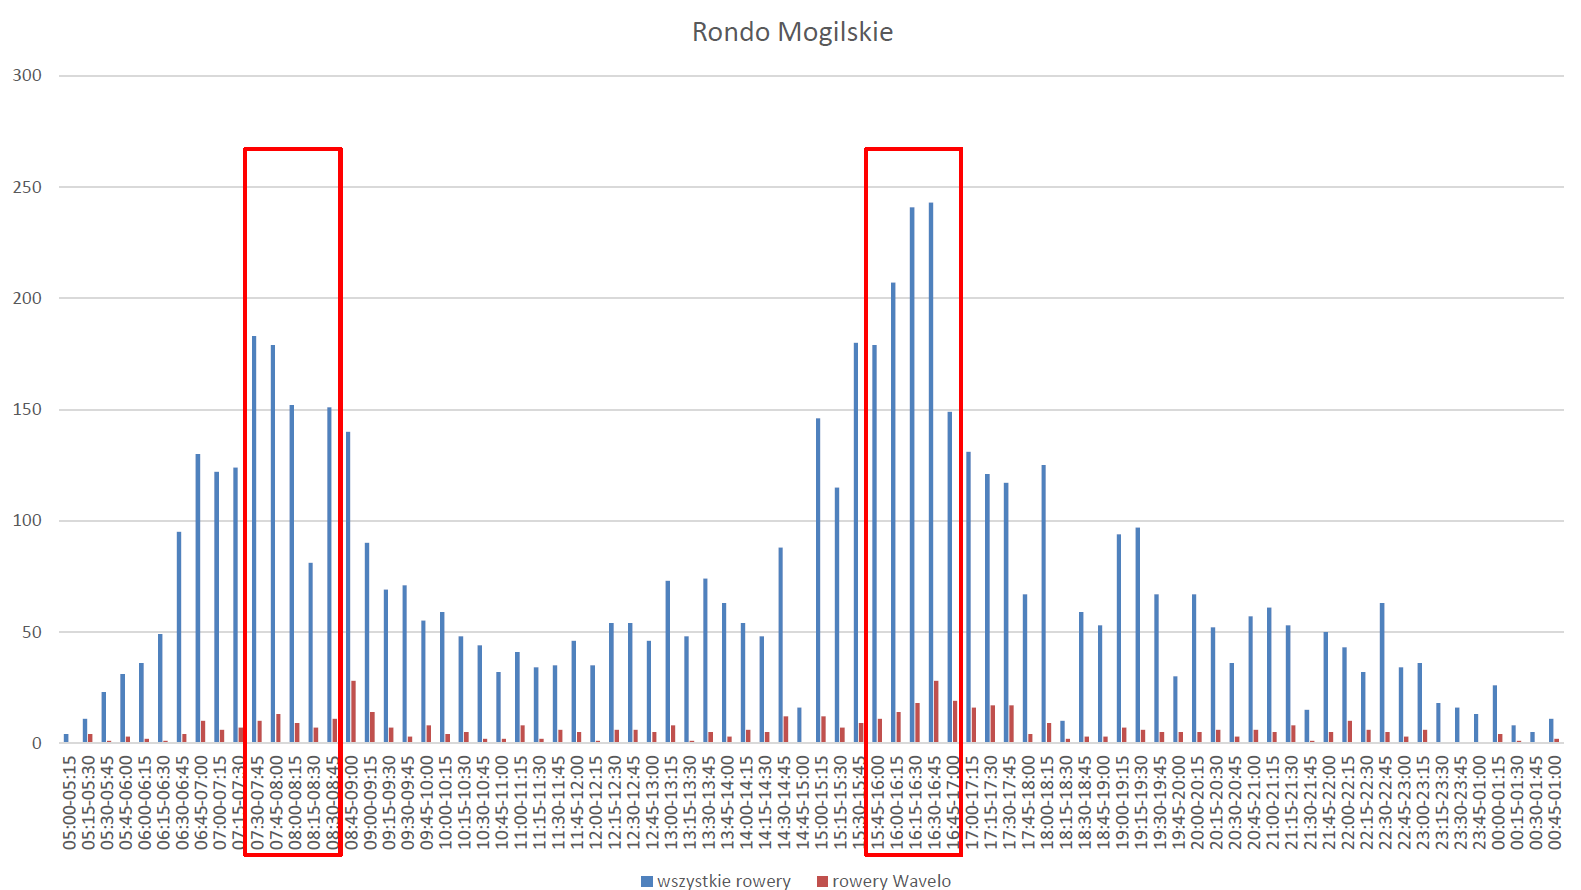
\includegraphics[width=\textwidth]{nat_ruchu_row}
\caption{[1]Natężenie ruchu rowerowego na Rondzie Mogilskim wg. Urzędu Miasta Krakowa (pomiar dokonany dnia 19.06.2018).}
\end{figure}
U podstaw niniejszego zjawiska leżą zróżnicowane przyczyny i nie wszystkie można wytłumaczyć powszechną modą na ekologię czy rosnącą popularnością roweru jako ogólnej formy rekreacji. Ważne aspekty, wpływające na wybór roweru jako środka komunikacji, to między innymi także takie kwestie jak możliwość bezproblemowego (w większości przypadków) dojazdu dokładnie do naszej destynacji, ekonomiczność takiego rodzaju komunikacji (jazda jest darmowa, jedynym wydatkiem jest kupno samego roweru), a w nierzadkich przypadkach i czasu (rower nie stoi w korkach, a jednocześnie jest dużo szybszy niż poruszanie się pieszo), czy korzyści zdrowotne wynikające z regularnego wysiłku fizycznego. Niemałym atutem roweru jest również jego łatwiejsze zaparkowanie – w centrach większych miast stojaki rowerowe są rozmieszczone całkiem gęsto i w zasadzie nigdy nie brakuje na nich miejsca, czego nie można powiedzieć o stanowiskach parkingowych dla samochodów. Te, oraz wiele innych przyczyn, pozwala zrozumieć dlaczego liczba amatorów bezsilnikowych jednośladów regularnie rośnie i nie wygląda na to by rosnąć miała przestać. Co istotniejsze nie tylko tych jeżdżących dla przyjemności w swoim czasie wolnym, ale także – a może przede wszystkim – tych korzystających z roweru jako zamiennika samochodu lub komunikacji zbiorowej. Tendencję tę można zauważyć zwłaszcza w miastach o bardzo dużym natężeniu ruchu samochodowego, co ułatwia wydedukowanie oczywistych zależności: w miastach odległości są względnie niewielkie, a powstające na głównych ciągach komunikacyjnych zatory w ruchu pojazdów mechanicznych, powodują znaczne wydłużenie czasu podróży przy użyciu tychże. Stąd rower całkiem często okazuje się wybawieniem, środkiem transportu, który zaoszczędza niemało czasu i niejako przy okazji daje okazję do poruszania się i spalenia palu kalorii. Dlatego też widok dużej ilości stojaków rowerowych ustawionych przy siedzibach największych firm nikogo nie dziwi. Wręcz przeciwnie – nie raz pracownicy jakiegoś przedsiębiorstwa potrafią wprost wypomnieć brak takiego udogodnienia.  
Obecna strategia każdego większego miasta – zwłaszcza europejskiego – opiera się niejako na stworzeniu jak największych możliwych udogodnień dla rowerzystów, jednocześnie starając się ograniczyć ruch samochodowy. Oba aspekty łączą się ze sobą w jedną spójną całość, a obrana przez miejskie władze ścieżka rozwoju nie jest podyktowana wyłącznie ekologią, ale także chłodną ekonomiczną kalkulacją. Metropolia, której drogi są permanentnie zakorkowane, w dłuższej (a czasem także i w krótszej) perspektywie czasu traci finansowo. Oczywiście straty te nie są bezpośrednie, a wynikają z odpływu mieszkańców, w efekcie czego spada liczba przedsiębiorstw, a koniec końców także i turystów.  Kraków nie chciał pozostać w tyle za innymi europejskimi miastami i również od kilku lat stara się inwestować w infrastrukturę rowerową, z gorszym lub lepszym skutkiem. Wprawdzie wdrażane i planowane inwestycje we wszelkiego rodzaju ścieżki rowerowe i innego typu udogodnienia nie zaspokajają znacznie szybciej rosnących potrzeb krakowskich rowerzystów, to jednak trzeba docenić fakt ich powstawania oraz zauważyć, że sieć tras już teraz jest całkiem przyzwoita. Efektem tego podróż z dowolnego miejsca w Krakowie przy pomocy bicykla nie jest już udręką i może być w dużej mierze realizowana po specjalnie wyznaczonym obszarze. Oczywiście lata zaniedbań powodują, że nie wszystko da się poprawić od razu, więc i w stolicy Małopolski nadal znajdują się białe plamy, gdzie teoretycznie dojazd rowerem umożliwia jedynie zwykła ulica, jednak takich miejsc systematycznie ubywa. Co najistotniejsze miejskie władze mocno skupiły się na tworzeniu ścieżek w najbardziej newralgicznych obszarach, dzięki czemu większość dużych skupisk ludzkich (gdzie na co dzień mieszka i sypia sporo mieszkańców) oraz dzielnic usługowo-handlowych czy też biznesowych (gdzie owi mieszkańcy pracują lub udają się na zakupy bądź relaks) jest ze sobą nad wyraz poprawnie skomunikowana pod względem rowerowym. \newline
Daje się jednak zauważyć, iż pomimo nie najgorszej infrastruktury, wielu krakowskich rowerzystów – często być może nieświadomie – nie wykorzystuje potencjału w niej drzemiącego. Widok rowerzysty poruszającego się po zwykłej drodze, podczas gdy istnieje alternatywna, wcale nie dłuższa ścieżka wytyczona specjalnie dla tego typu transportu, nie należy do rzadkości, pomimo faktu, iż rowerzysta ma obowiązek korzystania z drogi rowerowej, gdy ta jest poprowadzona bezpośrednio przy danej jezdni. A przecież taka sytuacja nie jest komfortowa ani dla użytkownika roweru, ani kierowcy samochodu, co więcej stanowi również dużo większe zagrożenie dla bezpieczeństwa rowerzysty. Niemałe jest także grono osób niezdecydowanych, dla których hasło „dojazd do pracy rowerem” lub podobne kojarzy się bardziej z koniecznością slalomu między samochodami, wdychaniem spalin i strachem przed potrąceniem, niż z oszczędnością czasu i pieniędzy. Tego typu ludzie również nie mają pełnej wiedzy na temat tego jak wygląda infrastruktura rowerowa w Krakowie, często przekonując się o tym dopiero po pierwszych przejazdach, metodą prób i błędów. Sytuacja ta wynika oczywiście ze sporej dynamiki rozwoju udogodnień dla rowerów, o której wspomniano wcześniej.
Trafnym staje się zatem pytanie: jak w łatwy sposób doinformować ludzi? Jak zachęcić ich do korzystania z rowerów? Rozwiązaniem wydaje się stworzenie czegoś w rodzaju swoistego przewodnika po infrastrukturze rowerowej Krakowa, dlaczego więc nie pójść krok dalej i nie stworzyć pełnoprawnej nawigacji rowerowej? Nie da się ukryć, że grupą społeczną, wśród której najprościej jest rozpropagować jakiś trend lub modę, jest grupa ludzi młodych, głównie przed 35 rokiem życia. W jaki sposób stworzyć u takich ludzi zainteresowanie? Oczywiście przy pomocy zawoalowania rozwiązania w kokon nowoczesnych rozwiązań, najlepiej więc by taka nawigacja była aplikacją na smartfony. To także poszerza dostępność rozwiązania, gdyż obecnie niemal każdy posiada smartfon. \newline
Nawigacja rowerowa w swym zamyśle ma więc nie tylko pomóc przeciętnemu rowerzyście w przemieszczaniu się po Krakowie, lecz także propagować taką formę transportu. Propagować i pomagać niezdecydowanym, tak by wybrali opcję rowerową. Wystarczy przecież rzut oka na wyznaczoną trasę pomiędzy interesującymi nas punktami i nagle okazuję się, że przejazd między nimi nie musi wiązać się z jazdą po ruchliwej ulicy. Niezwykle ważnym jest by aplikacja nie pozostała w tyle za szybkimi zmianami w topografii miasta, dlatego też musi być oparta o regularnie aktualizowane i niezawodne dane. Takimi bez wątpienia są dane tworzone przez instytucję, która ma bezpośredni wpływ na wygląd siatki ścieżek rowerowych w mieści, dlatego też aplikację opisaną w niniejszej pracy oparto na bazie danych ZTP.
